En esta tercer practica comenzaremos a trabajar con operaciones matematicas
entre las bandas del sateltica y en el uso de los resultados para obtener
relaciones empiricas con las variables biofisicas medibles en el terreno. Son
objetivos de las mismas

\begin{itemize}
    \item Poder calcular los indices de vegetacion a partir de las imágenes en
        reflectancia.
    \item Poder calcular la linea de suelo como parametro para calcular índices
        de vegetación.
    \item Poder realizar modelos empiricos que relacionen variables biofisicas
        medidas a campo con los indices calculados.
    \item Construir mapas a partir de los modelos empiricos antes mencionados.
\end{itemize}


\subsection{Calculo de indices entre bandas}
Comenzamos trabajando con el calculo de indices entre bandas. Para ello
utilizaremos lass lirberias \texttt{raster} y \texttt{RStoolbox}. Ademas para
poder usar mejores paletas de colores utilizaremos la libreria
\texttt{RColorBrewer}, sin embargo el uso de la misma es optativo. Por ultimo
puede ayudar cargar la libreria \texttt{rasterVis} para realizar algunos de los
graficos.

Comenzamos primer cargando la imagen desde el metadato y convirtiendola a
reflectancia entre cero y uno.

\begin{lstlisting}
    xml.2016 <- readMeta("raster_data/LC82240782016304/LC82240782016304LGN00.xml")
    ref.2016 <- stackMeta(xml.2016, quantity = "sre")
    scaleF <- getMeta(ref.2016,xml.2016, what = "SCALE_FACTOR")
    ref.2016 <- ref.2016 * scaleF
    ref.2016 <- ref.2016[[-1,]]
    names(ref.2016) <- c("blue","green","red","nir","swir1","swir2")
\end{lstlisting}

una vez cargada la imagen podemos realizar operaciones entre las bandas llamando
a cada una por separado. Veamos como ejemplo el calculo de NDVI\@.

\begin{exa}
    Calculo de NDVI a mano y grafico del mismo. 
    \begin{lstlisting}
    ndvi.2016 <- (ref.2016$nir-ref.2016$red)/(ref.2016$nir+ref.2016$red)
    cols = colorRampPalette(brewer.pal(9,"YlGn"))(256)
    plot(ndvi.2016, col=cols, zlim = c(0,1))
    \end{lstlisting}
    En este caso estamos
    \begin{itemize}
        \item Primero calculando el ndvi a mano.
        \item Segundo obteniendo la rampa de color con 16 valores entre amarillo
            y verde.
        \item Por ultimo graficando el ndvi, utilizando como colores dicha rampa
            y ajustandolo entre 0 y 1, es decir, los valores menores a 0 se
            mostraran todos del mismo color.
    \end{itemize}
    Obtenemos entonces
    \begin{figure}
    \begin{center}
        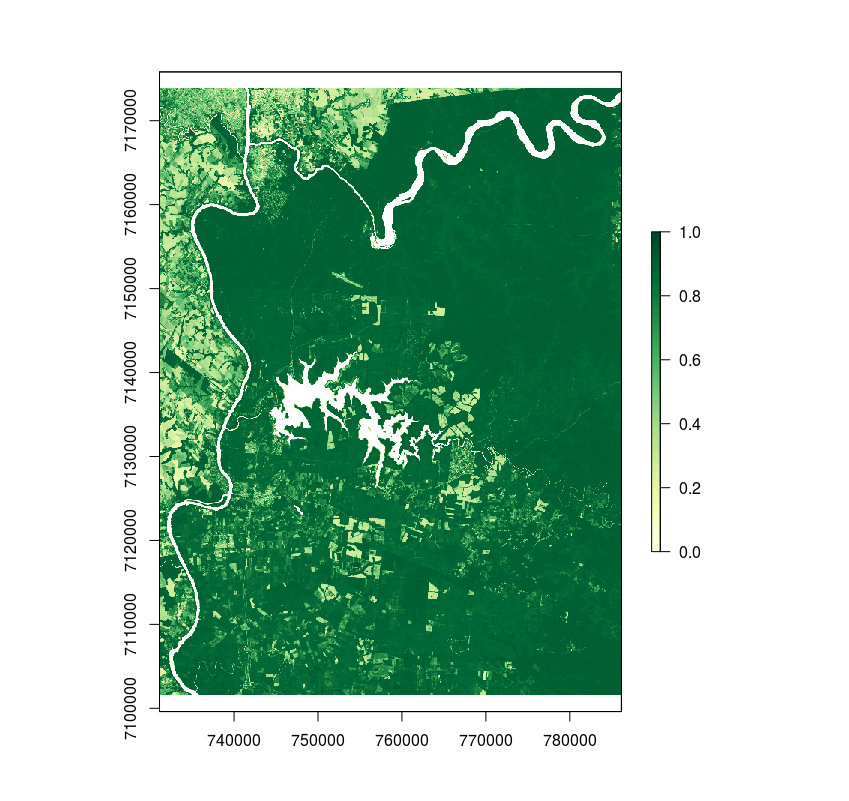
\includegraphics[scale=0.6]{ndvi_fig.png}
    \end{center}
    \caption{Mapa del NDVI en escala de verdes.}
    \label{fig:ndvifig}
    \end{figure}
    
\end{exa}

El paquete \texttt{RStoolbox} tiene varias herramientas que nos ayudan a
calcular los indices espectrales. Veamos por ejemplo como calcular el NDVI y el
EVI utilizando dicho paquete

\begin{exa}
    Para calcular los indices mediante la funcion spectralIndices debemos
    especificar con que raster trabajamos y que bandas corresponden a cada
    longitud de onda
    \begin{lstlisting}
    indices.2016 <- spectralIndices(ref.2016, 
                                    blue="blue", red="red", nir="nir", 
                                    indices=c("NDVI","EVI"))
    plot(indices.2016,col=cols, zlim=c(0,1))
    \end{lstlisting}
    En este caso, vemos que la funcion \texttt{espectralIndices} necesita al
    menos 3 parametros
    \begin{itemize}
        \item La imagen con la cual vamos a trabajar.
        \item A que zona del espectro corresponde cada banda.
        \item Los indices que queremos calcular
    \end{itemize}
     \begin{figure}
     \begin{center}
         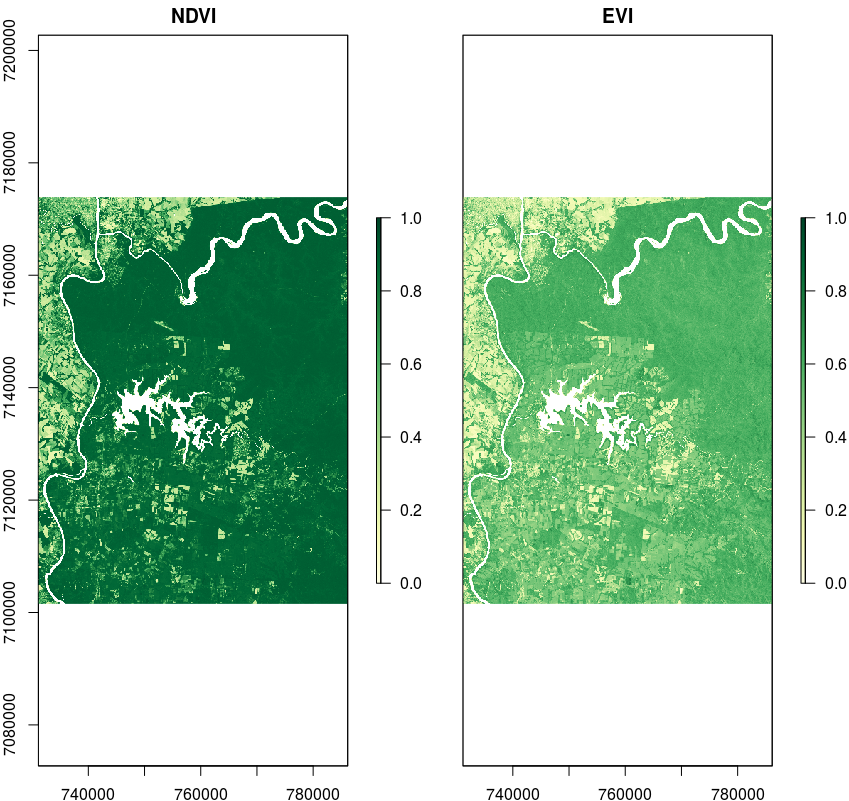
\includegraphics[scale=0.6]{evi-ndvi.png}
     \end{center}
     \caption{Graficos del EVI y el NDVI para la imagen seleccionada.}
     \label{fig:evi-ndvi}
     \end{figure}
     
\end{exa}

\begin{act}
    Calcule el NDVI y el EVI para el año 2000 utilizando la imagen landsat 7.
\end{act}

\begin{act}
    Calcule y grafique todos los indices posibles que involucren a las bandas
    roja y nir de landsat 8. 
\end{act}

\subsection{Calculo de la linea de suelo}

Algunos indices de vegetacion y una forma de extraer informacion util sobre las
imagenes satelitales es calcular la linea de suelo de la misma. Para hacerlo
debemos extraer la linea de los pixeles correspondientes a las zonas sin
cobertura vegetal en la imagen. Veamos como hacerlo utilizando la libreria
\texttt{landsat}

\begin{exa}
    Veamos ahora como calcular el tSAVI utilizando la linea de suelo obtenida a
    partir de la imagen. Para esto necesitaremos enmascarar las zonas con
    cobertura de agua y nubes. Veamos primer como hacer esto.
    \begin{lstlisting}
    mask.2016 <- raster("raster_data/LC82240782016304/LC82240782016304LGN00_cfmask.tif")
    masked.2016 <- mask(ref.2016, mask=mask.2016, inverse=TRUE,
                        maskvalue=0, updatevalue=255)
    masked.2016[masked.2016<=0] <- 255
    \end{lstlisting}
    de esta forma enmascaramos todos los valores con nubes, agua y donde la
    reflectancia obtenida es cero con el valor 255.
    Calculamos ahora la linea de suelo y la mostramos en un scatterplot
    \begin{lstlisting}
    bsl.2016 <- BSL(as.matrix(masked.2016$red), as.matrix(masked.2016$nir),
                    method="quantile")
    plot(ref.2016$red, ref.2016$nir)
    abline(bsl.2016$BSL,col="red")
    \end{lstlisting}
    Obtenemos como resultado el grafico de la linea de suelo. Podemos consultar
    los demas parametros imprimiendo la variable \texttt{bsl.2016}.
    \begin{figure}
    \begin{center}
        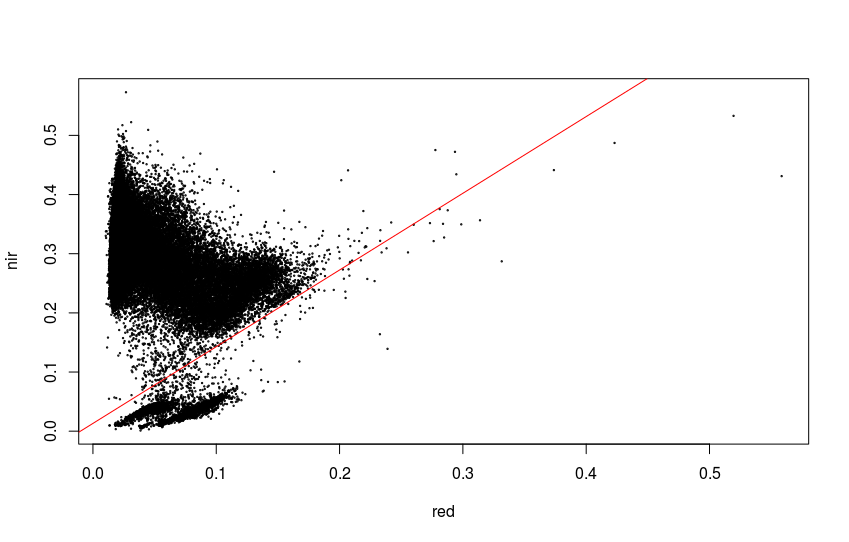
\includegraphics[scale=0.6]{soil.png}
    \end{center}
    \caption{Linea de suelo sobre el scatterplot nir-red}
    \label{fig:soil}
    \end{figure}
    
\end{exa}

\begin{act}
    Calcule el tSAVI utilizando la linea de suelo obtenida arriba.
\end{act}

\begin{act}
    Vuelva a obtener la linea de suelo sin enmascarar la imagen y dibujo el
    scatterplot con la misma y la anterior. Que problema encuentra.
\end{act}

\begin{act}
    Obtenga la linea de suelo y calcule el indice tSAVI para la imagen del año
    2000.
\end{act}

\subsection{Estimacion de parametros biofisicos}

Finalmente, veamos como se puede obtener datos biofisicos a partir de los
indices de vegetacion calculados. De esta forma podremos generar mapas de
porcentaje de cobertura, productividad, etc.

\begin{act}
    Cargue la capa vectorial del muestreo de variables biofisicas
    \texttt{muestreo.shp} y haga una extraccion de los valores de NDVI
    correspondientes a dichos puntos. Guarde estos valores en un dataframe
    llamado \texttt{muestreo}.
\end{act}

\begin{exa}
    Comenzamos calculando el ndvi para el año 2016, y utilizando la capa
    muestreo hacemos una extraccion estadistica sobre la misma.
    \begin{lstlisting}
    tor <- readOGR(dsn="vector_data/", layer="muestreo")
    datos <- extract(ndvi.2016,vector)
    DF <- data.frame(vector@data,datos)
    end{lstlisting}
    Veamos como ajustar con R un modelo lineal a nuestro modelo. Para esto
    comencemos haciendo un analisis visual con la funcion \texttt{ggpairs}.
    \begin{lstlisting}
    ggpairs(muestreo,diag=list(continuous="barDiag"))
    \end{lstlisting}
    Obtendremos un grafico que presenta los scatterplots entre las bandas, su
    correlacion e histogramas.
    Veamos en el mismo que la superficie cubierta por vegetacion varia
    linealmente con el NDVI\@. Por lo tanto utilizaremos estos para hacer un
    ajuste de nuestro modelo.
    \begin{lstlisting}
        lm.2016 <- lm(fcover~ndvi, data=muestreo)
        plot(muestreo$ndvi, mustreo$fcover)
        abline(lm.2016, col="red")
        summary(lm.2016)
    \end{lstlisting}
    de esta forma veremos los parametros de nuestro ajuste, y graficaremos al
    mismo en un scatterplot.

    Para aplicar el modelo a nuestro raster hacemos
    \begin{lstlisting}
        fcover.2016 <- predict(ndvi.2016,lm.2016)
        plot(fcover.2016)
    \end{lstlisting}
    Obteniendo el mapa de abajo.
\end{exa}

\begin{act}
    Genere los modelos de lai, fapar y fcover para el año 2016 y con los mismos
    realice mapas de dichas variables.
\end{act}

\begin{act}
    Utilizando los modelos obtenidos para 2016 aplique los mismos para obtener
    los mapas de lai, fapar y fcover del año 2000. Que suposicion esta
    haciendo?
\end{act}

\begin{act}
    * Utilizando la funcion spectralIndices y ggpairs, analice si hay otro indice
    que ajuste que correlacione mejor con las alguna de las varibles biofisicas
    medidas a campo.
\end{act}

